\chapter{Introdução}

%Contextualização android vai dominar precisamso programar pra ele
A tendência do mercado de dispositivos  handset é aumentar segundo IDC  é
experado um crescimento de 32.7\% na produção\cite{idc:a}. O sistema operacional
android é o líder dominando 75\% desse mercado com mais de 162 milhões de
smartphones produzidos e embarcados com android\cite{idc:b}. Baseados nesses
dados podemos concluir que existe uma damanda no desenvolvimento de novos 
aplicativos que agregem valor à esses aparelhos.
% é preciso que tenha   - Design Principles.
Para produzir aplicativos de qualidade é necessário aplicar boas práticas de
desenvolvimento de software. Levando em consideração que a linguagem de
programação usado para o desenvolvimento na plataforma android é a Java, é
natural que se aplique as práticas definidas pelos princípios de projeto
orientado a objetos. Esses princípios guiam o desenvolvedor em como definir a
estrutura interna do software afetando diretamente as características  de
qualidade como manutenabilidade, performance e outras\cite{tempero-di}.

Os padrões de projeto são aplicados na engenharia de software como forma de
reproduzir  soluções  para problemas recorrentes melhorando a manutenabilidade e
o reuso de componentes de software\cite{gof} então o uso de padrões de projetos
é um meio de aplicar esses princípios. Segundo \citeonline{pressman}, ``A
interface com o usuário pode ser considerada o elemento mais importante de
um sistema ou produto baseado em computador``, tendo em vista isso, será tratado
nesse trabalho  os padrões para desenvolvimento da camada de apresentação de 
em aplicativos android.

\section{Motivação}

A motivação para a execução desta pesquisa sugiu da participação do autor em
projetos para desenvolvimento de aplicativos android em uma instituição de
pesquisa e desenvolvimento localizada em manaus. O comprometimento com a
qualidade promoveu o uso de ferramentas de código aberto para monitoração da
qualidade dos projetos além do processo de testes adotado pela empresa. Com uma
equipe composta por mais de 30 desenvolvedores produzindo aplicativos com
diversas finalidades houve a necessidades de padronização da arquitetura.

\section{Problematização}
Dado que existem uma vasta diversidade de padrões de proejtos a serem aplicados
no desenvolvimento de software, Qual padrão de projeto é aplicável para o
desenvolvimento da camada de apresentação de aplicativos android para melhorar a
qualidade do produto final?

\section{Hipótese}

O padrão de projeto Model-View-Presenter é aplicável no desenvolvimento da
camada de apresentação de aplicativos android, gerando um aumento da qualidade
do produto final.

% ---
% Capitulo de revisão de literatura
% ---
\section{Objetivos}

Este trabalho fará um estudo sobre a arquitetura de aplicativos android com o
propósito de melhorar a qualidade desses softwares reduzindo riscos relacionados
as mudanças que acontecem durente o ciclo de desenvolvimento e promova a
reutilização de componentes e que permita o incremento de funcionalidades com
baixo impacto. Este estudo fornecerá insumos para que os desenvolvedores possam
ter uma visão geral da aplicabilidade dos padrões de projetos e analisar quais
técnicas contribuem para o seu trabalho. Este trabalho tem como meta:

\begin{itemize}
\item Estudar os padrões de projeto que podem ser usados para a implementação da
camada de apresentação de um aplicativo android.
\item Avaliar os componentes do  framework android identificando seus papéis e
responsabilidades de acordo com os padões estudados levando  em consideração
características que podem dificultar a aplicação dos padrões. 
\item Identificar os impactos nas características de qualidade do aplicativo de acordo
com o paradigma da Orientação a objetos.
\item Elaborar um referência de implementação para a  camada de apresentação de um
aplicativo android utilizando padrões de projetos.
\end{itemize}

\section{Trabalhos Relacionados}

Na dissertação de \citeonline{turk} é feita uma análise dos impactos na
qualidade ao aplicar cinco padrões de projetos em um software de comunicação
TCP/IP. Os resultados do trabalho citado mostram que a qualidade do software
aumenta ao aplicar padrões de projetos sendo que o principal atributo de
qualidade aferida é a manutenabilidade.

\section{Contribuições}


Tendo em vista que padrões de projetos descrevem soluções genéricas, este
trabalho tem como principal contribuiçãouma interpretação do padrão de projeto
Model-View-Presenter proporcionando uma referência prática dentro framework
android.

A diversidade de projetos de software torna difícil inferir se as métricas
podem ser consideradas um paramêtro para determinar a qualidade. Para validar a
aplicabilidade do padrão MVP métricas orientadas a objetos foram usadas
dentro do contexto do framework android, contribuindo com mais uma estudo dessas
métricas acrescentando algo para a ciência. rsrs

\section{Organização do Trabalho}

Será descrito a metodologia, definicão do projeto, experimentos, conclusões.


\chapter{Metodologia}

Esta pesquisa se caracteríza como aplicada pois tem fins práticos ao realizar
uma revisão na literatura existente sobre orientação a objetos e seus princípios
bem como referências sobre padrões de projetos para proporcionar o embasamento
que auxiliará na identificação dos componetes do android que podem assumir as
responsabilidades definidas nos padrões e definir como implementa-los.

Para validar a hipótese apresentada neste trabalho a pesquisa terá uma
abordagem quantitativa através da análise de dados estatistícos de métricas 
que expresssam atributos de qualidade em software orientado a objetos. O
conjunto de métricas a serem usadas nessa validação será o elaborado por
\citeonline{cksuite}.

Essas medidas serão coletadas através de um procedimento experimental em
laboratório utilizando um processo iterativo-incremental para executar
refatorações no código do objeto de estudo afim de introduzir o padrão de
projeto Model-View-Presenter e a cada iteração será feita a coleata das
métricas. Para executar esse processo será identificado um conjunto de
funcionalidades que o aplicativo atende, relaciondas com a camada de
apresentação com a qual o usuário interage.



\section{Objeto de Estudo}


O projeto a ser refatorado será o aplicativo de Contatos do
android\footnote{https://github.com/android/platform_packages_apps_contacts} que é um dos aplicativos básicos pré-instalados com o sistema
operacional. Este projeto é opensource mantido pelo  The Android Open Source
Projeto suportado pela Google com contribuições de desenvolvedores do mundo
todo.(qual é a licença do projeto).

Os critérios para a escolha do objeto de estudo são:

\begin{enumerate}
  \item Tamanho/Complexidade - Um projeto muito complexo iria inviabilizar a
  pesquisa devido ao esforço para fazer a refatoração. Métricas coletadas
  apartir de projetos simples e triviais não forneceriam dados suficientes para
  uma análise satisfatória. (o que foi usado para medir a complexidade. e qual
  o tamanho do objeto de estudo).
  \item Código Aberto - Além de permitir o acesso ao código fonte sem
  limitações para a pesquisa, tem a contribuição de vários desenvolvedores com
  experiência e formação em programação diversificada que se refletem no código fonte.
  \item Origem do projeto - A escolha de um aplicativo mantido sobre o mesmo
  ``guarda-chuva'' que o sistema operacional android foi feita com o intuito de
  fazer a pesquisa em um código fonte que expressasse as técnicas e práticas de
  programação difundidas nesse ecosistema.
\end{enumerate}

\section{Processo de Experimentos}


A Figura \ref{processo_experimentacao} demonstra as atividades do processo de
experimentação adotado:
\begin{figure}[!h]
	\centering
	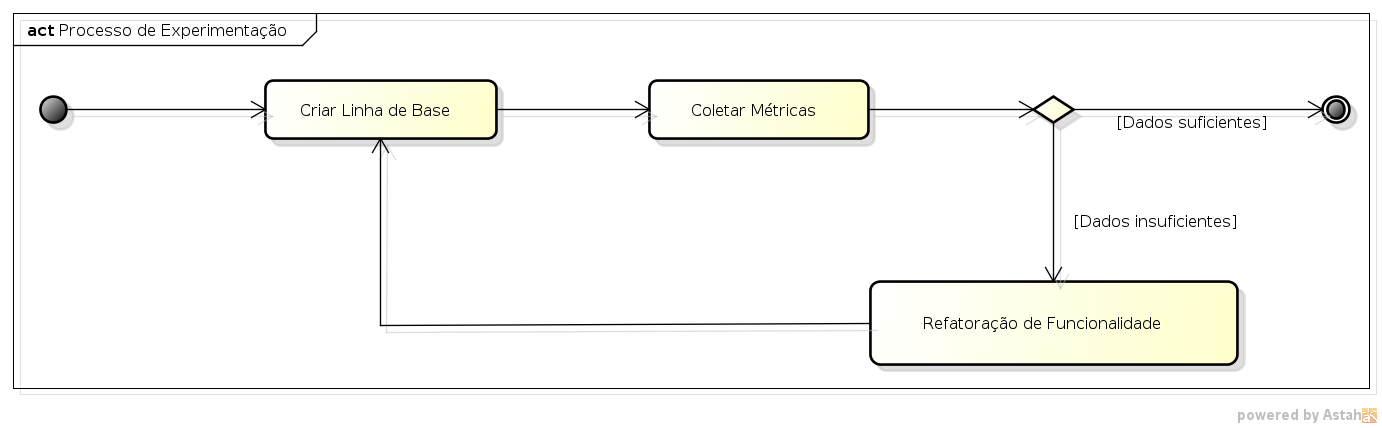
\includegraphics[scale=0.5]{img/processo_experimentacao.png}
	\caption{Processo de Experimentação Fonte: Próprio Autor}
	\label{processo_experimentacao}
\end{figure}

\begin{description}
\item[Criação uma linha de base] - Delimitar um marco do estado do código no
repositório.
\item[Refatoração Incremental] Esta atividade tem como objetivo aplicar os
padrões em uma funcionalidade do aplicativo.
\item[Coleta de Métricas] Este passo tem como objetivo fazer a coleta
das métricas do código apartir de uma revisão em que se encontra no repositório
para fazer a avaliação dos efeitos da refatoração na qualidade do código.
\end{description}

Esta pesquisa se propõe a executar três iterações.

\section{Ferramentas}

Para elaborar uma documentação da implementação de referências usando será usada
a notação UML v2 com o uso da ferramento Astah. O código será versionado no
Github onde será feito o gerenciamento das linhas de base. As ferramentas a
serem utilizadas para a refatoração, IDE Eclipse(Juno) com plugin ADT v21. As
métricas serão coletadas com o programa
ckjm\footnote{http://www.spinellis.gr/sw/ckjm/}.

**** Salientar que tudo que for feito neste trabalho é reproduzivel estará tudo
disponível no github.

